\documentclass[conference]{IEEEtran}

% ── Encoding & Language ────────────────────────────────────────────
\usepackage{iftex}
\ifPDFTeX
  \usepackage[utf8]{inputenc}
  \usepackage[T5]{fontenc}
\else
  \usepackage{fontspec}
  \defaultfontfeatures{Ligatures=TeX}
  \setmainfont{Latin Modern Roman}
\fi
\usepackage[vietnamese,english]{babel}

% ── Math ──────────────────────────────────────────────────────────
\usepackage{amsmath,amssymb}
\usepackage{bm}

% ── Graphics & Tables ─────────────────────────────────────────────
\usepackage{graphicx}
\graphicspath{{figures/}}
\usepackage{booktabs}
\usepackage{multirow}
\usepackage{array}
\usepackage{float}

% ── Hyperlinks ────────────────────────────────────────────────────
\usepackage[hidelinks]{hyperref}

% ── Caption ───────────────────────────────────────────────────────
\usepackage{caption}

% ── Bibliography ──────────────────────────────────────────────────
\usepackage{cite}

% ── Misc ──────────────────────────────────────────────────────────
\usepackage{xcolor}
\usepackage{enumitem}

\newcommand{\sys}{\textit{InternHub}}

% ══════════════════════════════════════════════════════════════════
\begin{document}

\title{Ứng Dụng Tư Duy Tính Toán Trong Xây Dựng Hệ Thống Gợi Ý Phỏng Vấn IT Cá Nhân Hóa Dựa Trên Knowledge Tracing}

\author{
  \IEEEauthorblockN{Mai Dương Hải Đăng}
  \IEEEauthorblockA{Khoa Khoa học và Kỹ thuật Thông tin\\
    Trường Đại học Công nghệ Thông tin, ĐHQG-HCM\\
    Thành phố Hồ Chí Minh, Việt Nam\\
    24520253@gm.uit.edu.vn}
  \and
  \IEEEauthorblockN{Tạ Gia Khiêm}
  \IEEEauthorblockA{Khoa Khoa học và Kỹ thuật Thông tin\\
    Trường Đại học Công nghệ Thông tin, ĐHQG-HCM\\
    Thành phố Hồ Chí Minh, Việt Nam\\
    24520805@gm.uit.edu.vn}
  \and
  \IEEEauthorblockN{Nguyễn Sỹ Huỳnh}
  \IEEEauthorblockA{Khoa Khoa học và Kỹ thuật Thông tin\\
    Trường Đại học Công nghệ Thông tin, ĐHQG-HCM\\
    Thành phố Hồ Chí Minh, Việt Nam\\
    24520716@gm.uit.edu.vn}
  \and
  \IEEEauthorblockN{Nguyễn Ngọc Nam}
  \IEEEauthorblockA{Khoa Khoa học và Kỹ thuật Thông tin\\
    Trường Đại học Công nghệ Thông tin, ĐHQG-HCM\\
    Thành phố Hồ Chí Minh, Việt Nam\\
    24521114@gm.uit.edu.vn}
}

\maketitle

% ── Abstract ──────────────────────────────────────────────────────
\begin{abstract}
Bài báo này trình bày quá trình áp dụng tư duy tính toán (Computational Thinking -- CT) để thiết kế và xây dựng \sys{}, một hệ thống luyện phỏng vấn IT cá nhân hóa tích hợp Knowledge Tracing (KT). Thông qua bốn bước CT -- \textit{phân rã} (decomposition), \textit{nhận dạng mẫu} (pattern recognition), \textit{trừu tượng hóa} (abstraction), và \textit{thiết kế thuật toán} (algorithm design) -- nhóm đã chuyển hóa bài toán thực tế phức tạp thành một pipeline khả thi: xây dựng question bank 2{,}122 câu cho ba vai trò Data Analyst/Scientist/Engineer, mô phỏng 1{,}000 người dùng tổng hợp với $\sim$40{,}000 tương tác, huấn luyện và so sánh các mô hình BKT, DKT, và SAKT, cuối cùng tích hợp vào ứng dụng web hoàn chỉnh. Kết quả thực nghiệm cho thấy DKT-Quality đạt PR-AUC~=~0.907 và RMSE~=~0.355 (tốt nhất trong nhóm neural), với PR-AUC Gain~=~0.087 so với baseline. Hệ thống triển khai thành công kiến trúc 2-Stage Branching CAT và cơ chế cập nhật skill vector KT(70\%)~+~EMA(30\%), chứng minh tính khả thi của việc ứng dụng CT để giải quyết bài toán giáo dục thực tế.
\end{abstract}

\begin{IEEEkeywords}
Tư duy tính toán, Knowledge Tracing, hệ thống gợi ý, phỏng vấn IT, học thích nghi
\end{IEEEkeywords}

% ══════════════════════════════════════════════════════════════════
\section{Giới Thiệu}
\label{sec:intro}

Tư duy tính toán (Computational Thinking -- CT) là tập hợp các kỹ năng tư duy giúp con người phân tích và giải quyết vấn đề theo cách mà máy tính có thể hỗ trợ thực thi \cite{wing2006computational}. CT không chỉ là lập trình -- đó là quá trình phân rã vấn đề phức tạp, nhận ra các mẫu lặp lại, trừu tượng hóa các chi tiết không cần thiết, và thiết kế thuật toán có thể tổng quát hóa.

Bài báo này trình bày cách nhóm vận dụng bốn trụ cột CT để giải quyết bài toán thực tế: \textit{Làm sao cá nhân hóa việc luyện phỏng vấn IT cho từng ứng viên theo trình độ thực tế của họ?}

Thị trường IT tại Việt Nam đang phát triển mạnh, nhưng hơn 70\% ứng viên chưa chuẩn bị đủ kỹ năng kỹ thuật trước phỏng vấn \cite{topdev2024}. Các nền tảng hiện có (LeetCode, HackerRank) chủ yếu tập trung vào thuật toán, thiếu nội dung cho ba vai trò dữ liệu phổ biến: Data Analyst (DA), Data Scientist (DS), Data Engineer (DE), và không theo dõi được trạng thái kiến thức của người học theo thời gian.

Giải pháp đề xuất -- \sys{} -- là hệ thống tích hợp Knowledge Tracing \cite{corbett1994knowledge}, chấm điểm LLM, và giao diện web React, được thiết kế hoàn toàn theo phương pháp CT từ phân tích bài toán đến triển khai.

% ══════════════════════════════════════════════════════════════════
\section{Tư Duy Tính Toán: Khung Lý Thuyết}
\label{sec:ct}

Theo Wing \cite{wing2006computational}, CT bao gồm bốn thành phần cốt lõi:

\textbf{(1) Phân rã (Decomposition):} Chia bài toán lớn thành các bài toán con có thể giải quyết độc lập.

\textbf{(2) Nhận dạng mẫu (Pattern Recognition):} Tìm ra các quy luật, điểm tương đồng giữa các bài toán hoặc dữ liệu.

\textbf{(3) Trừu tượng hóa (Abstraction):} Tập trung vào các thông tin cốt lõi, bỏ qua chi tiết không cần thiết để xây dựng mô hình tổng quát.

\textbf{(4) Thiết kế thuật toán (Algorithm Design):} Xây dựng chuỗi các bước rõ ràng, lặp lại được để giải quyết bài toán.

Trong \sys{}, nhóm áp dụng bốn trụ cột này theo trình tự có hệ thống như minh họa ở Hình~\ref{fig:ct_pipeline}.

\begin{figure}[H]
  \centering
  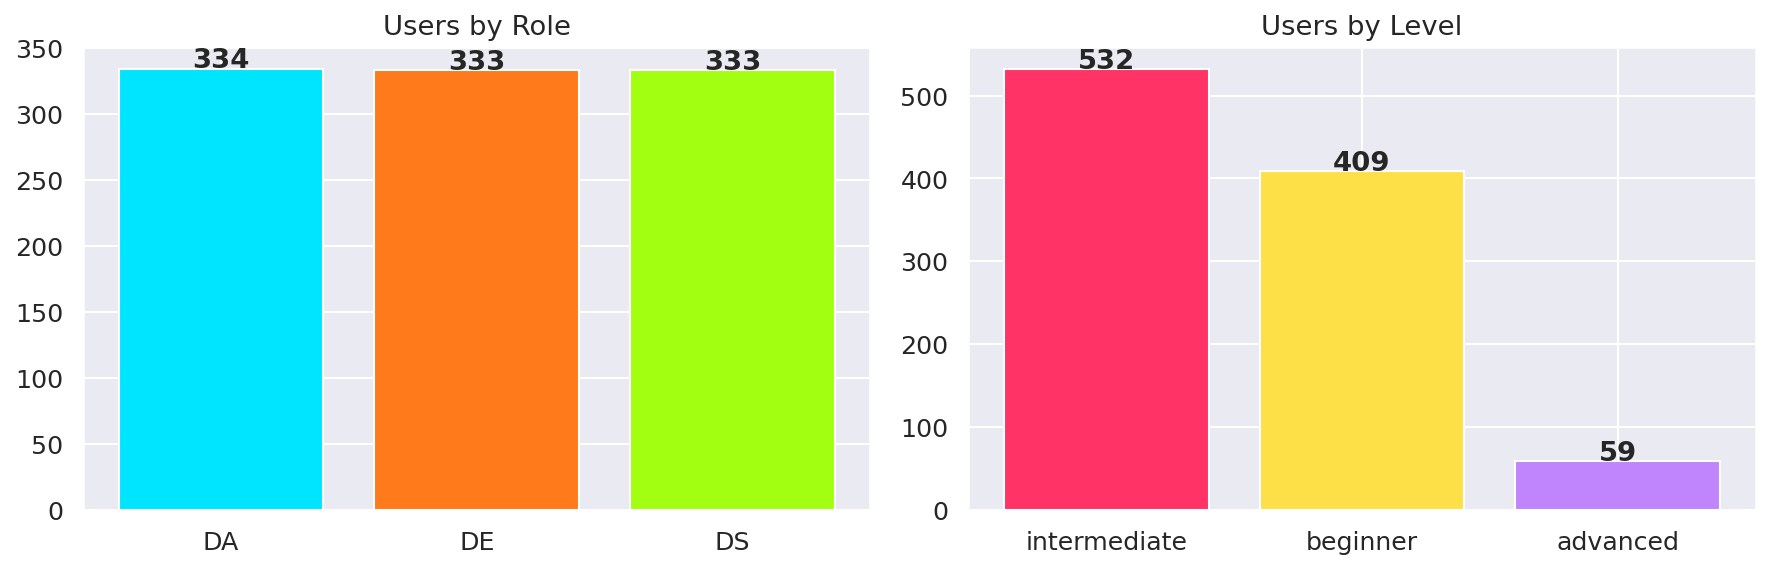
\includegraphics[width=0.95\columnwidth]{eda_user_distribution.png}
  \caption{Phân phối người dùng mô phỏng theo vai trò (DA/DS/DE) -- kết quả của bước Phân rã vai trò nghề nghiệp.}
  \label{fig:ct_pipeline}
\end{figure}

% ══════════════════════════════════════════════════════════════════
\section{Áp Dụng CT Vào Thiết Kế \sys{}}
\label{sec:apply_ct}

\subsection{Bước 1 -- Phân rã bài toán}

Bài toán ``luyện phỏng vấn IT cá nhân hóa'' được phân rã thành 5 bài toán con độc lập:

\begin{enumerate}[leftmargin=*,label=\arabic*.]
  \item \textbf{Bài toán nội dung:} Xây dựng question bank đa dạng, phủ đủ kỹ năng.
  \item \textbf{Bài toán dữ liệu:} Thu thập/mô phỏng lịch sử tương tác của người học.
  \item \textbf{Bài toán theo dõi:} Mô hình hóa trạng thái kiến thức (Knowledge Tracing).
  \item \textbf{Bài toán gợi ý:} Chọn câu hỏi phù hợp theo trình độ hiện tại.
  \item \textbf{Bài toán giao diện:} Xây dựng ứng dụng tương tác hoàn chỉnh.
\end{enumerate}

Mỗi bài toán con được giao cho một module riêng biệt trong hệ thống (Hình~\ref{fig:architecture}).

\begin{figure}[H]
  \centering
  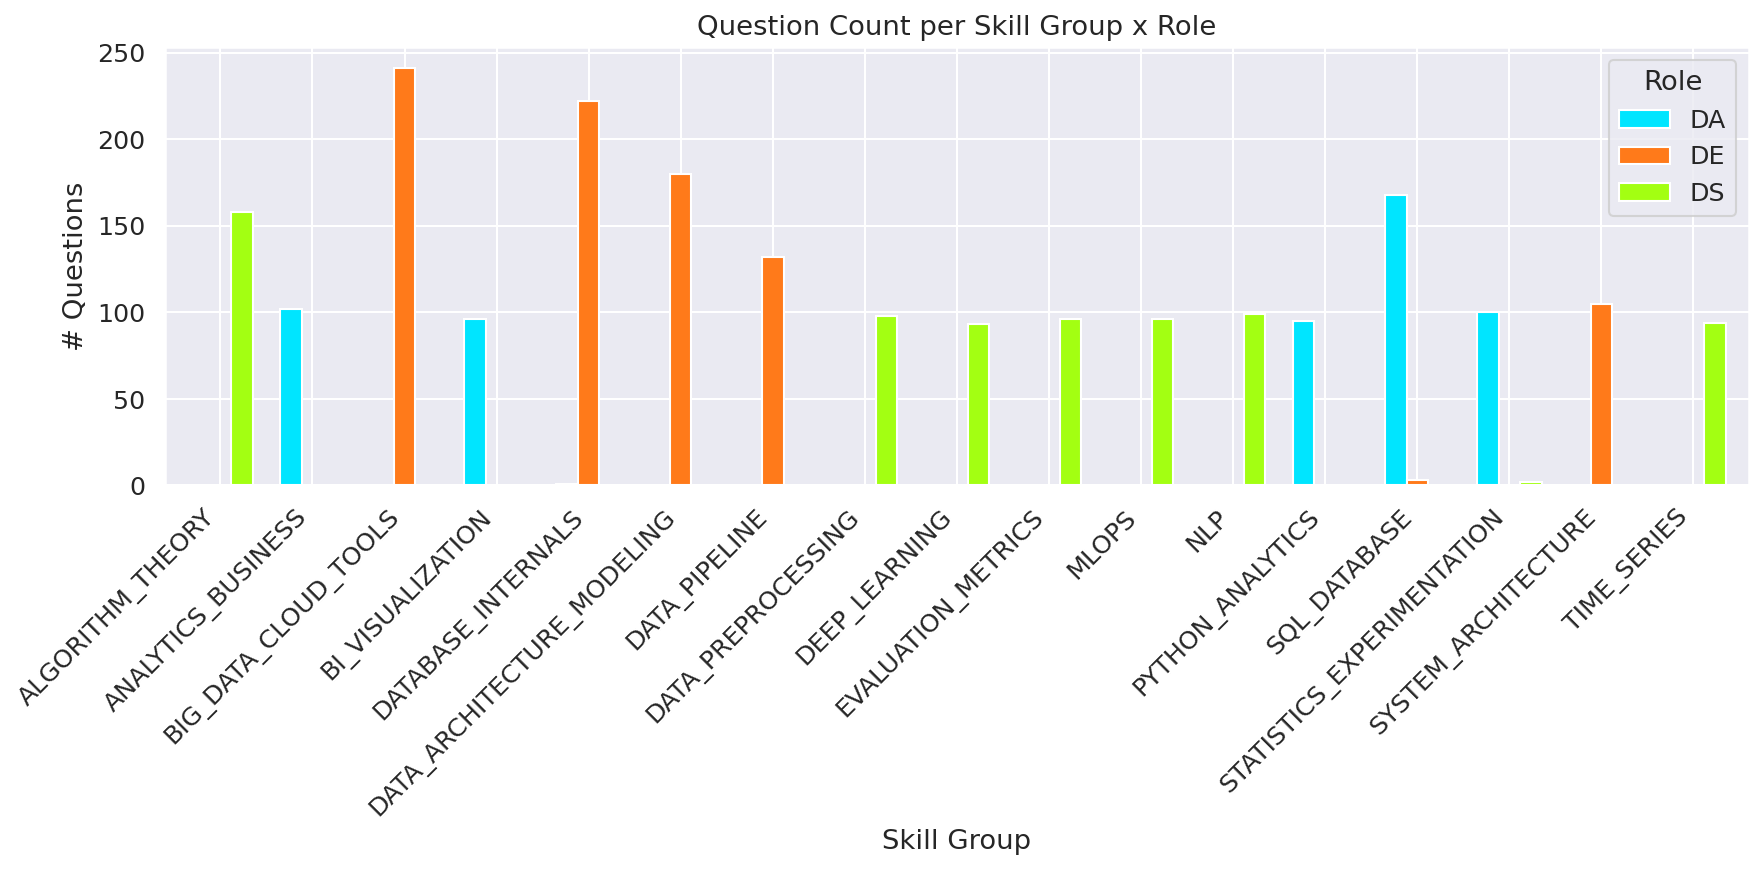
\includegraphics[width=0.95\columnwidth]{eda_qbank_skill_coverage.png}
  \caption{Phủ kỹ năng của question bank theo 17 KC -- minh chứng cho kết quả phân rã bài toán nội dung.}
  \label{fig:architecture}
\end{figure}

\subsection{Bước 2 -- Nhận dạng mẫu}

Qua phân tích dữ liệu EDA, nhóm nhận ra các mẫu quan trọng:

\textbf{Mẫu học tập:} Điểm của người dùng tăng đơn điệu theo thời gian (learning curve dốc lên), đặc biệt rõ ở 10 tương tác đầu (Hình~\ref{fig:learning_curve}). Điều này xác nhận cần một cơ chế ``adaptive'' thay vì tĩnh.

\textbf{Mẫu phân nhóm:} Người dùng tự nhiên phân thành ba nhóm trình độ (WEAK/MID/STRONG) dựa trên pass ratio trong 5 câu đầu, với ranh giới rõ ràng tại ngưỡng 40\% và 70\%.

\textbf{Mẫu câu hỏi:} Câu hỏi CODING và PRACTICE có độ phân biệt cao hơn (AUC per-KC cao hơn) so với câu hỏi THEORY đơn thuần.

\begin{figure}[H]
  \centering
  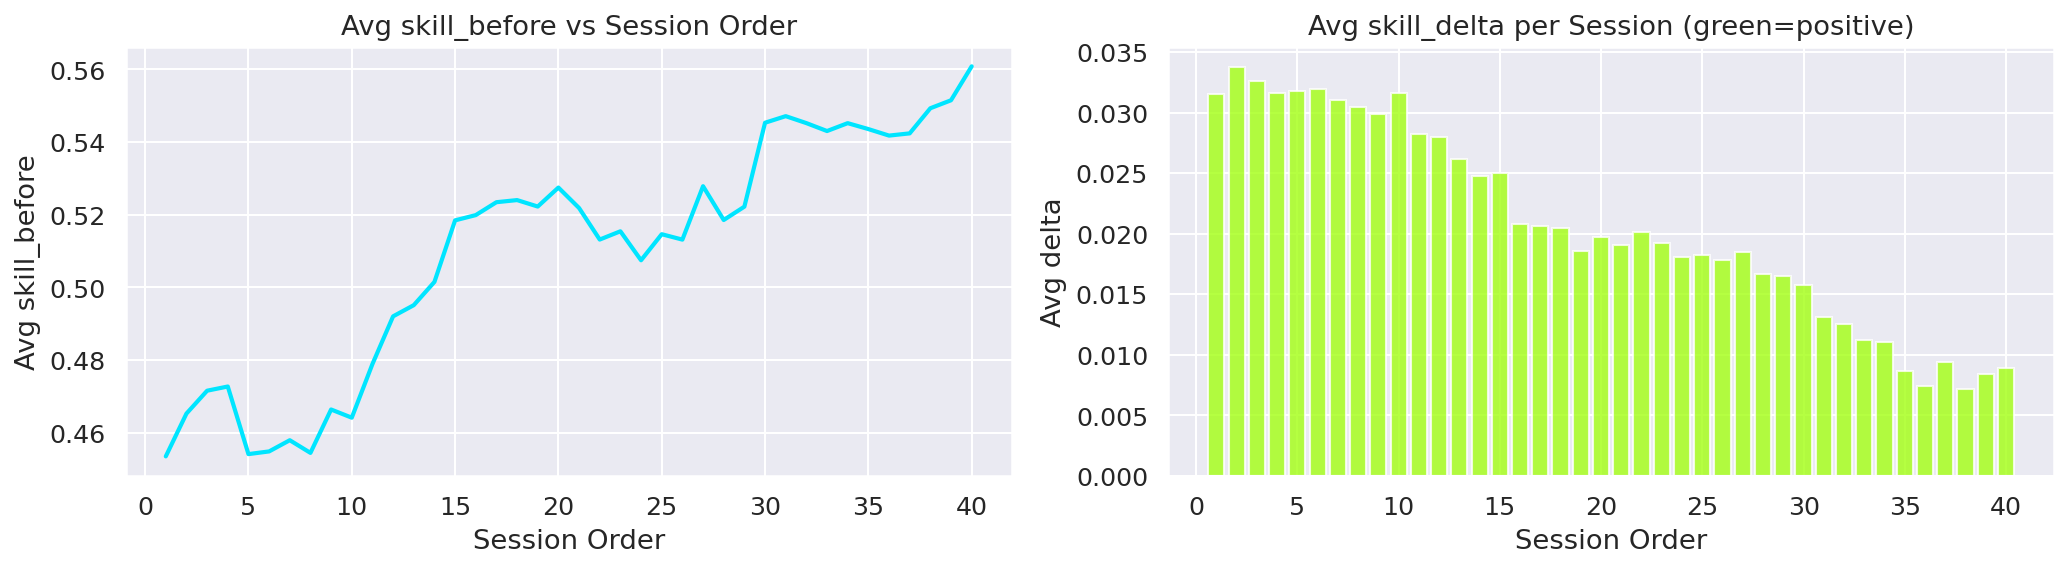
\includegraphics[width=0.95\columnwidth]{eda_learning_curve.png}
  \caption{Learning curve trung bình theo số tương tác -- mẫu học tập tăng trưởng ổn định.}
  \label{fig:learning_curve}
\end{figure}

\subsection{Bước 3 -- Trừu tượng hóa}

Từ bài toán cụ thể, nhóm xây dựng các mô hình trừu tượng:

\textbf{Knowledge Component (KC):} Trừu tượng hóa ``kỹ năng'' thành 17 KC chuẩn hóa dưới dạng vector $\bm{\theta} \in [0,1]^{17}$, độc lập với loại câu hỏi hay ngôn ngữ diễn đạt.

\textbf{Skill Vector:} Mỗi người dùng được biểu diễn bằng vector năng lực $\bm{\theta}_u \in \mathbb{R}^{17}$, là trừu tượng hóa toàn bộ lịch sử tương tác thành một điểm trong không gian kỹ năng.

\textbf{Interaction Sequence:} Lịch sử học tập được trừu tượng hóa thành chuỗi $(q_t, r_t)_{t=1}^{T}$ -- cặp (câu hỏi, kết quả) -- đủ để KT model học được dynamics mà không cần lưu trữ nội dung câu trả lời thực sự.

\textbf{IRT Parameters:} Độ khó câu hỏi được trừu tượng hóa thành tham số $b \in \{0.30, 0.55, 0.80\}$ tương ứng EASY/MEDIUM/HARD, thay vì dùng độ dài hay từ ngữ câu hỏi.

\subsection{Bước 4 -- Thiết kế thuật toán}

Nhóm thiết kế ba thuật toán cốt lõi:

\subsubsection{Thuật toán 2-Stage Branching CAT}

\begin{enumerate}[leftmargin=*,label=\arabic*.]
  \item Stage 1: Chọn 7 câu -- mỗi KC một câu, phủ đủ 17 KC (DA/DE lặp 2 KC top).
  \item Tính pass ratio từ kết quả Stage 1.
  \item Phân nhánh: WEAK ($< 0.4$) $\to$ ưu tiên câu dễ; STRONG ($\geq 0.7$) $\to$ ưu tiên câu khó; MID $\to$ intermediate.
  \item Stage 2: Chọn 3 câu ưu tiên KC yếu (score $< 0.5$), độ khó theo routing.
\end{enumerate}

\subsubsection{Thuật toán Cập Nhật Skill Vector}

Sau mỗi tương tác, skill vector được cập nhật theo công thức blend KT--EMA:
\begin{equation}
  \hat{\bm{\theta}}_{t+1} =
  \begin{cases}
    \bm{\theta}_{\text{EMA}} & \text{nếu } |history| < 3 \\
    0.7 \cdot \bm{\theta}_{KT} + 0.3 \cdot \bm{\theta}_{\text{EMA}} & \text{ngược lại}
  \end{cases}
  \label{eq:blend}
\end{equation}

trong đó $\bm{\theta}_{KT}$ là dự đoán từ mô hình DKT và $\bm{\theta}_{\text{EMA}}$ là Exponential Moving Average của lịch sử điểm.

\subsubsection{Thuật toán Chấm Điểm Tự Động (Local Rubric)}

Cho câu hỏi mở, thuật toán chấm điểm local dùng 4 lớp có trọng số:
\begin{equation}
  S = 0.50 \cdot S_{\text{eval}} + 0.25 \cdot S_{\text{kw}} + 0.15 \cdot S_{\text{rubric}} + 0.10 \cdot S_{\text{len}}
\end{equation}

với $S_{\text{eval}}$ là điểm khớp evaluation points (Jaccard $\geq 0.5$), $S_{\text{kw}}$ là keyword matching, $S_{\text{rubric}}$ là rubric matching, và $S_{\text{len}}$ là điểm độ dài câu trả lời.

% ══════════════════════════════════════════════════════════════════
\section{Xây Dựng Dữ Liệu}
\label{sec:data}

\subsection{Question Bank}

Do thiếu dataset công khai cho phỏng vấn IT, nhóm xây dựng question bank bằng pipeline LLM tự động: Gemini Flash sinh câu hỏi, GPT-4o viết đáp án tham khảo, Claude Haiku đánh giá chất lượng. Kết quả: 2{,}122 câu hỏi phân bổ theo ba vai trò và 17 KC (Hình~\ref{fig:qbank_dist}).

\begin{figure}[H]
  \centering
  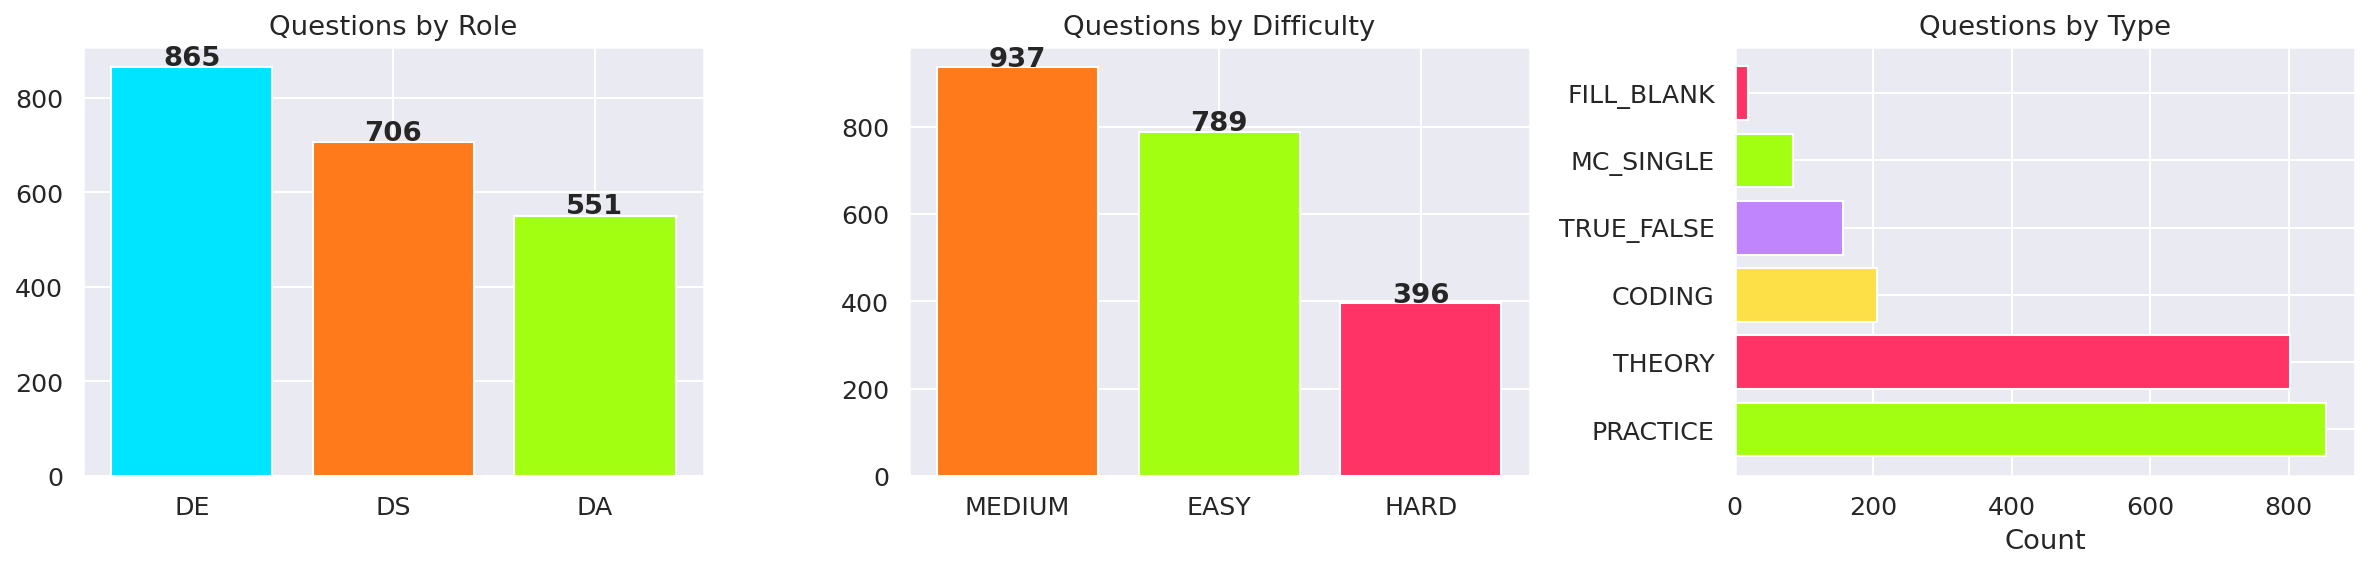
\includegraphics[width=0.95\columnwidth]{eda_qbank_distribution.png}
  \caption{Phân phối câu hỏi theo vai trò và loại câu hỏi trong question bank.}
  \label{fig:qbank_dist}
\end{figure}

\subsection{Dữ Liệu Mô Phỏng IRT}

Nhóm áp dụng mô hình IRT 3-Parameter Logistic (3PL) \cite{embretson2000item} để mô phỏng hành vi 1{,}000 người dùng ảo:
\begin{equation}
  P(r=1|\theta, a, b, c) = c + (1-c) \cdot \frac{1}{1+e^{-a(\theta-b)}}
\end{equation}

Kết quả: $\sim$40{,}000 tương tác, phân chia 70/15/15 (train/val/test), pass rate 82.5\%, không data leakage giữa train và test (Hình~\ref{fig:sparsity}).

\begin{figure}[H]
  \centering
  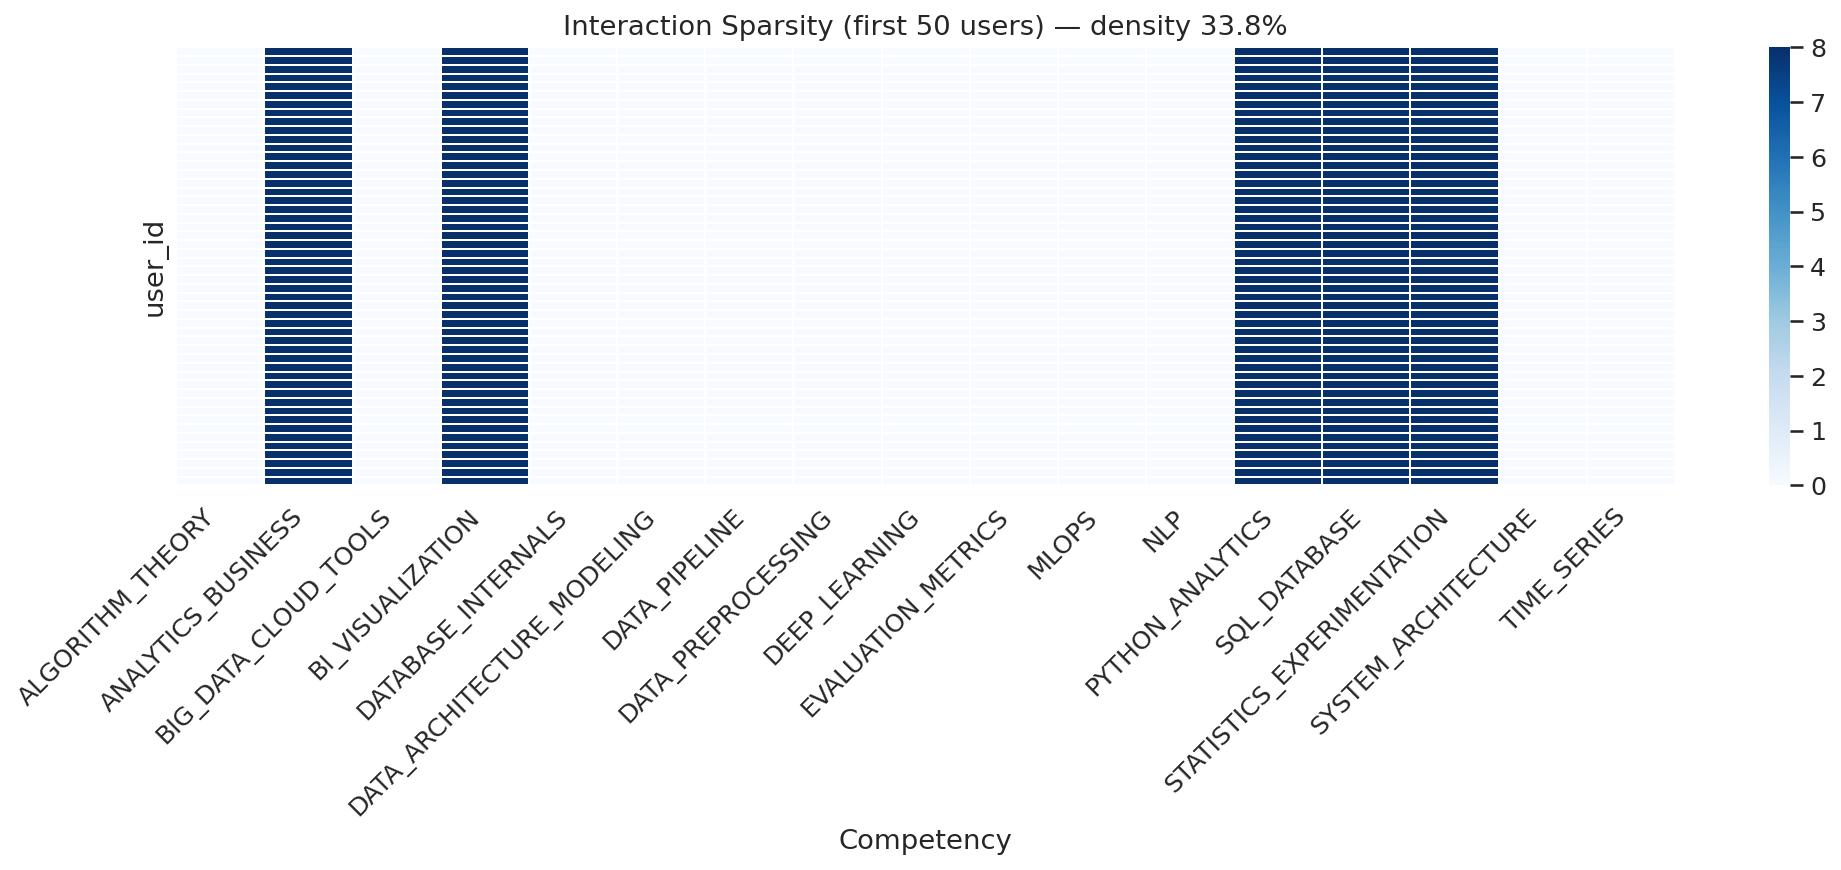
\includegraphics[width=0.95\columnwidth]{eda_sparsity_matrix.png}
  \caption{Ma trận thưa (sparsity) user--question. Mật độ tương tác đồng đều theo thiết kế.}
  \label{fig:sparsity}
\end{figure}

% ══════════════════════════════════════════════════════════════════
\section{Mô Hình Knowledge Tracing}
\label{sec:kt}

\subsection{Ba Họ Mô Hình}

\textbf{BKT} \cite{corbett1994knowledge}: Mô hình Markov ẩn (HMM) 4 tham số per KC. Cập nhật trạng thái theo Bayes sau mỗi quan sát. Ưu điểm: diễn giải được, huấn luyện nhanh (54.8s). Hạn chế: giả định KC độc lập.

\textbf{DKT} \cite{piech2015deep}: Mạng LSTM học biểu diễn ẩn từ chuỗi tương tác. Đầu vào $(q_t, r_t)$ one-hot, đầu ra xác suất đúng cho tất cả KC trong một forward pass -- quan trọng cho real-time recommendation.

\textbf{SAKT} \cite{pandey2019self}: Thay LSTM bằng self-attention, học mối liên hệ trực tiếp giữa các KC liên quan trong lịch sử. Nhanh hơn DKT do song song hóa (11.0s training).

\subsection{Đóng Góp: DKT với Quality Label}

Nhóm đề xuất biến thể \textbf{DKT-Quality}: thay nhãn nhị phân $r_t \in \{0,1\}$ bằng điểm chất lượng liên tục $r_t \in [0,1]$ và chuyển loss sang MSE:
\begin{equation}
  \mathcal{L}_{\text{quality}} = \frac{1}{T}\sum_{t=1}^{T}(r_t - \hat{y}_t)^2
\end{equation}

Điều này cung cấp gradient phong phú hơn, phản ánh tốt hơn mức độ thành thạo thực tế.

% ══════════════════════════════════════════════════════════════════
\section{Thực Nghiệm và Kết Quả}
\label{sec:exp}

\subsection{Môi Trường}

Thực nghiệm trên Kaggle Notebooks: CPU Intel Xeon 2-core 13GB RAM, GPU NVIDIA Tesla T4 16GB, PyTorch 2.6, Python 3.12, seed 42.

\subsection{Kết Quả Ablation Study}

\begin{table}[H]
  \centering
  \caption{Kết quả so sánh 8 cấu hình trên tập test (150 users, 6{,}065 tương tác)}
  \label{tab:results}
  \resizebox{\columnwidth}{!}{%
  \begin{tabular}{lcccc}
    \toprule
    \textbf{Mô hình} & \textbf{ROC-AUC} & \textbf{PR-AUC} & \textbf{PR-AUC Gain} & \textbf{RMSE} \\
    \midrule
    Baseline         & 0.500 & 0.820 & 0.000 & 0.384 \\
    BKT              & \textbf{0.677} & 0.905 & 0.085 & 0.374 \\
    DKT-Binary       & 0.666 & 0.905 & 0.085 & 0.375 \\
    DKT-Quality$^*$  & 0.672 & \textbf{0.907} & \textbf{0.087} & \textbf{0.355} \\
    SAKT-Binary      & 0.668 & 0.903 & 0.083 & 0.373 \\
    SAKT-Quality$^*$ & 0.667 & 0.904 & 0.084 & 0.356 \\
    DKT-Deep         & 0.669 & 0.906 & 0.086 & 0.375 \\
    SAKT-Deep        & 0.670 & 0.906 & 0.086 & 0.373 \\
    \bottomrule
  \end{tabular}%
  }
  \vspace{2pt}
  \small{$^*$: sử dụng quality label liên tục, tốt nhất trong nhóm.}
\end{table}

\begin{figure}[H]
  \centering
  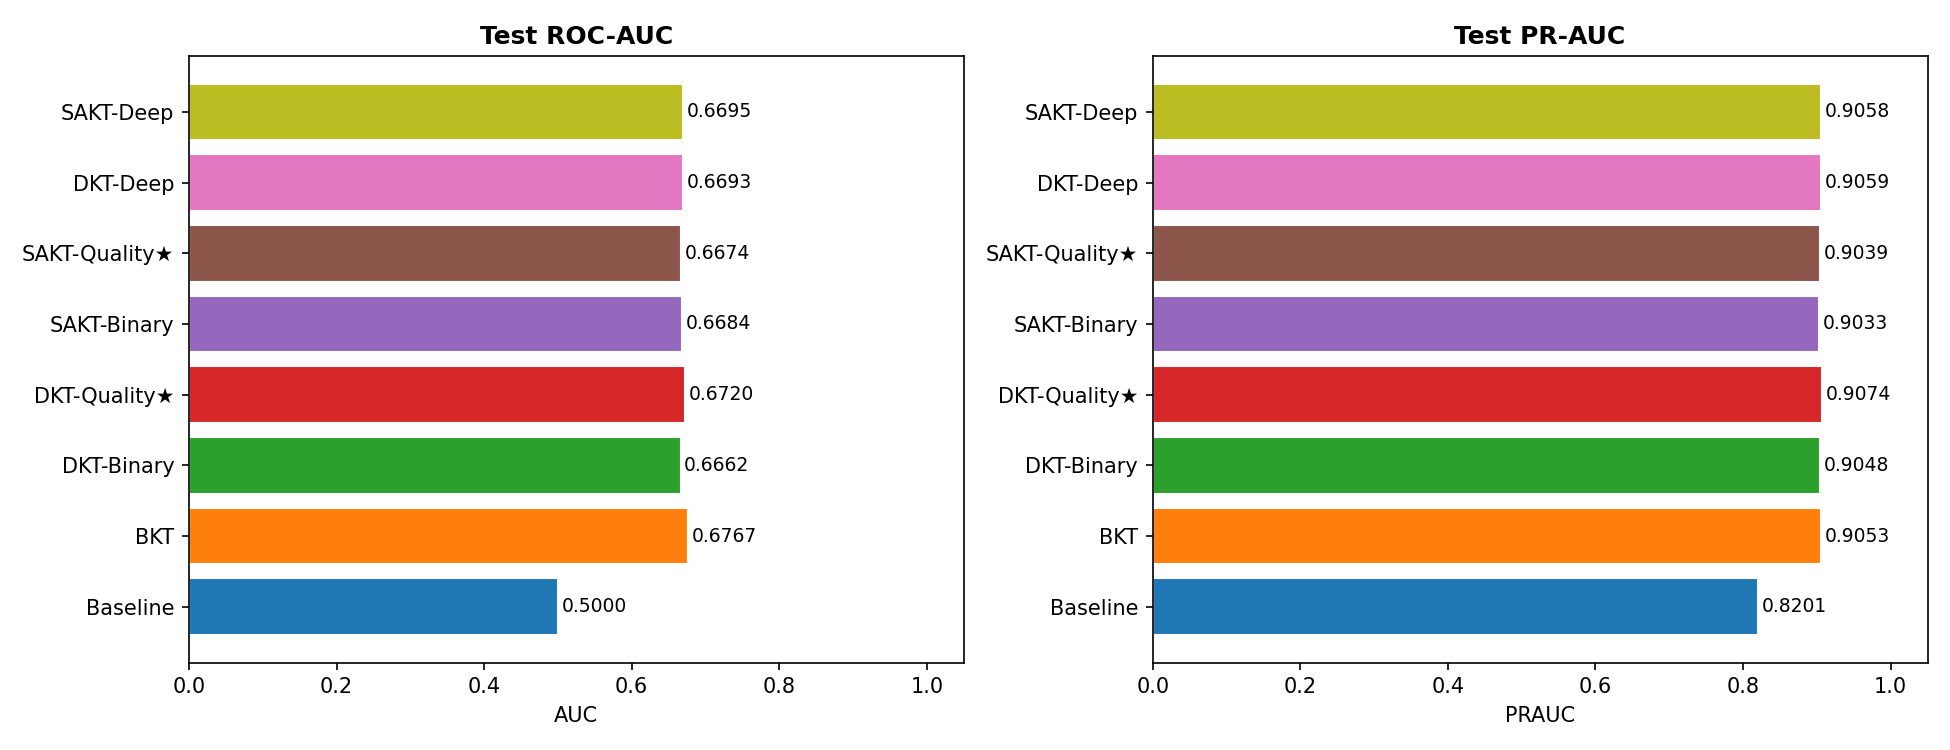
\includegraphics[width=0.95\columnwidth]{ablation_bar.png}
  \caption{So sánh ROC-AUC và PR-AUC của 8 cấu hình -- DKT-Quality đạt PR-AUC cao nhất.}
  \label{fig:ablation}
\end{figure}

\subsection{Phân Tích Chi Tiết}

\textbf{Hiệu quả của KT:} Tất cả 7 mô hình vượt baseline rõ rệt -- PR-AUC Gain đạt 0.083--0.087, xác nhận lịch sử tương tác mang thông tin dự đoán thực sự.

\textbf{Hiệu quả của quality label:} DKT-Quality đạt RMSE thấp nhất (0.355 vs 0.375 của DKT-Binary), tốt hơn 5.3\%. Gradient liên tục giúp mô hình học biểu diễn trạng thái kiến thức phong phú hơn.

\textbf{BKT và simulation bias:} BKT đạt ROC-AUC cao nhất (0.677) do data được sinh bởi mô hình IRT -- cùng inductive bias với BKT. Trên dữ liệu thực, DKT/SAKT dự kiến vượt trội hơn.

\begin{figure}[H]
  \centering
  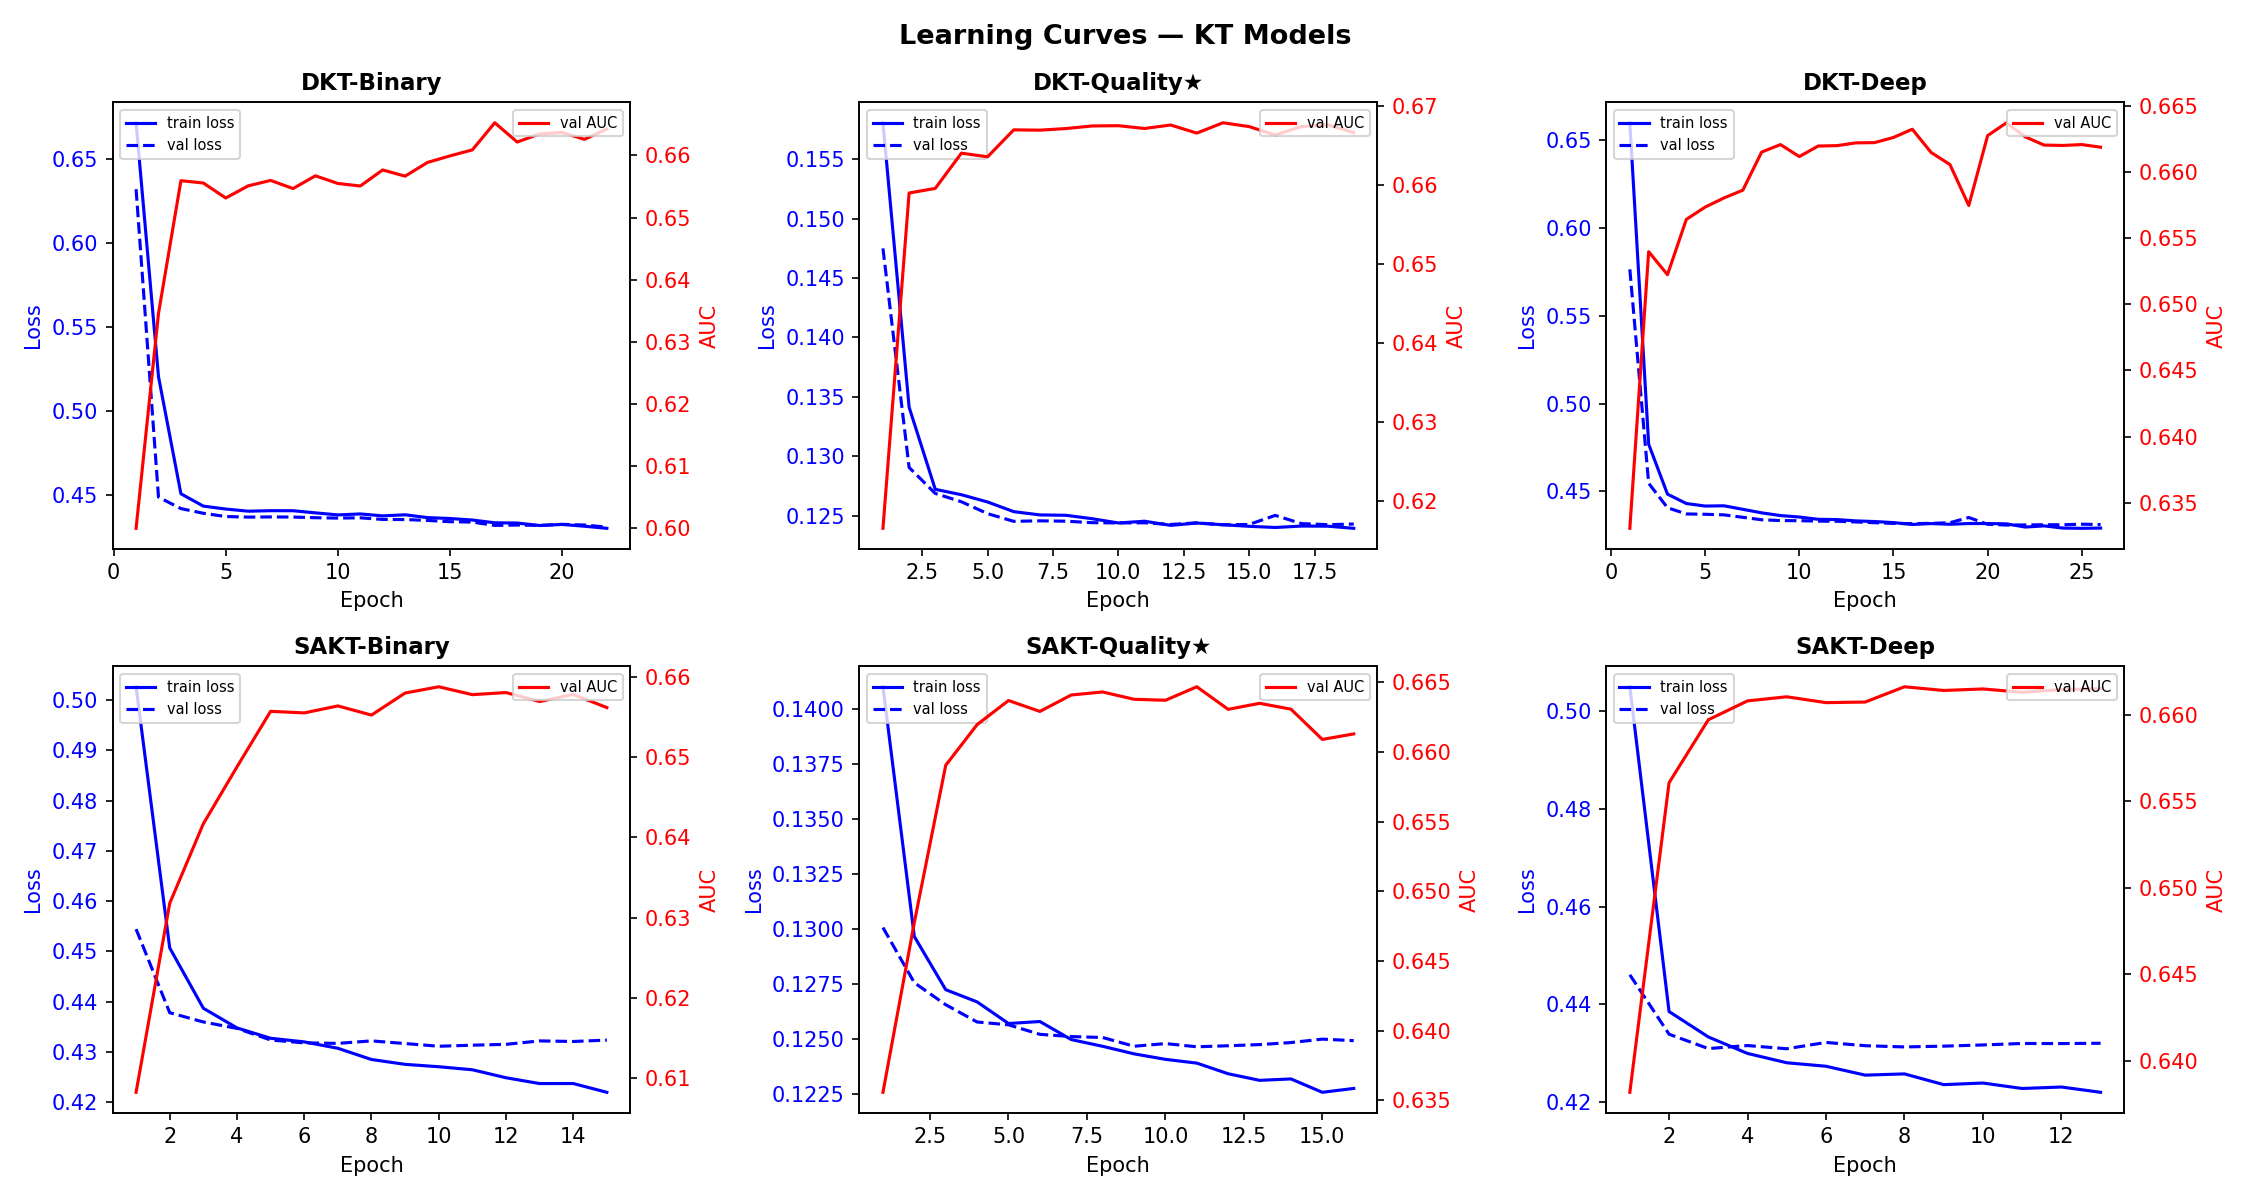
\includegraphics[width=0.95\columnwidth]{learning_curves.png}
  \caption{Learning curves của 6 mô hình neural -- DKT-Quality hội tụ nhanh và ổn định nhất.}
  \label{fig:learning_curves}
\end{figure}

\begin{figure}[H]
  \centering
  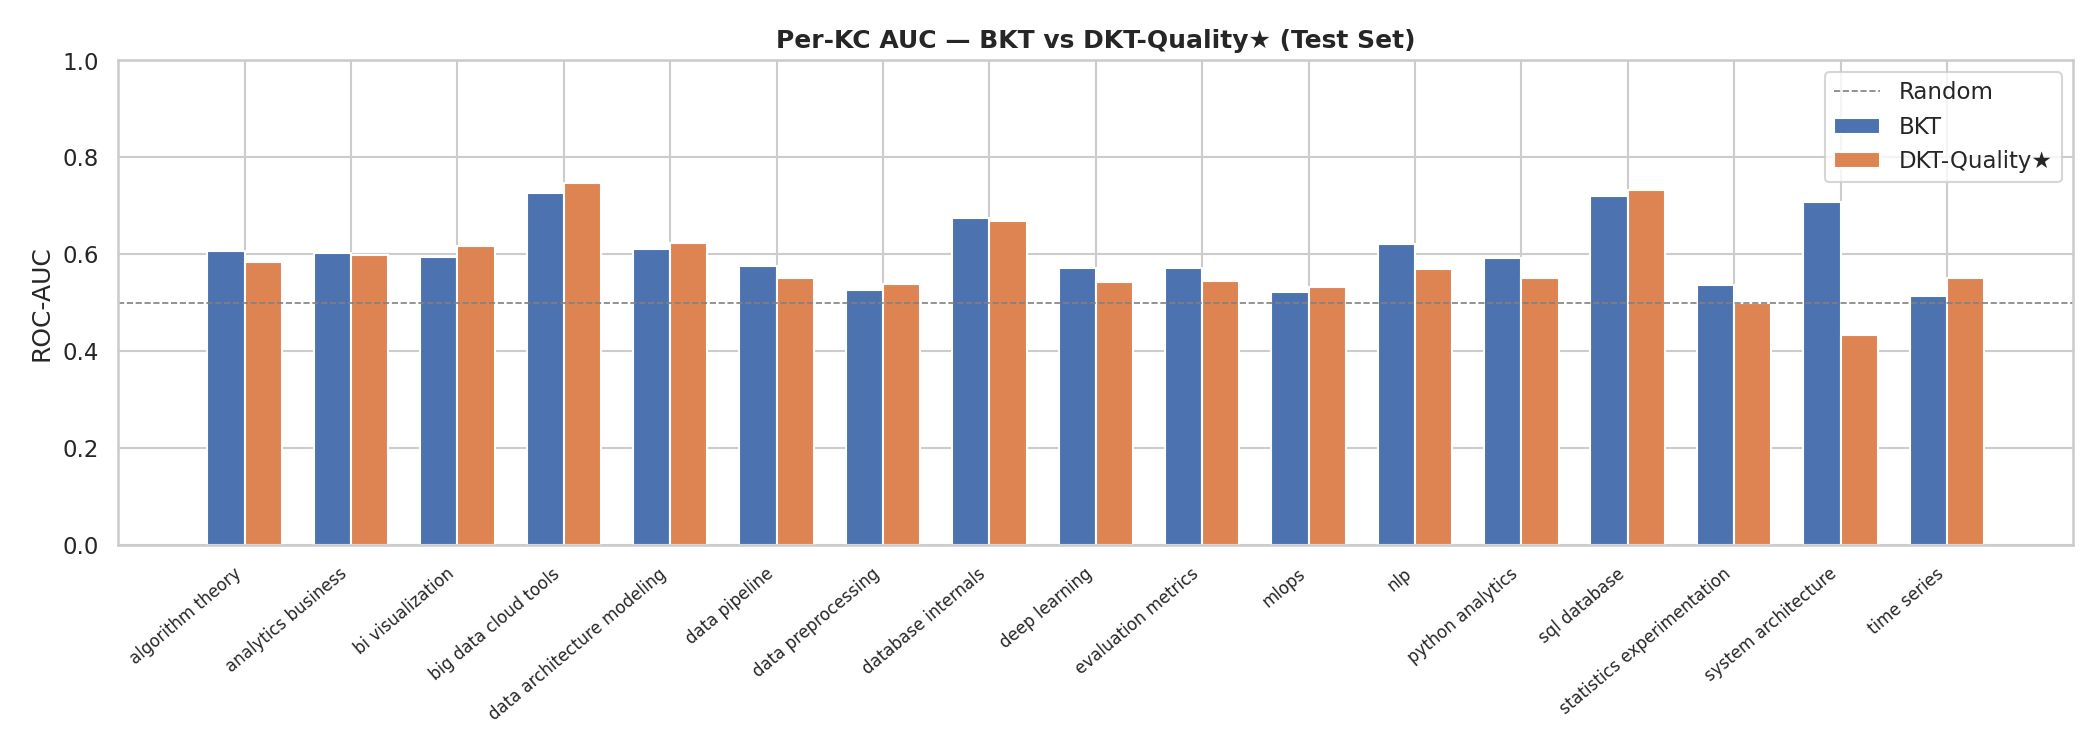
\includegraphics[width=0.95\columnwidth]{per_kc_auc.png}
  \caption{ROC-AUC theo từng KC -- mô hình phân biệt tốt ở các KC có nhiều dữ liệu.}
  \label{fig:per_kc}
\end{figure}

\begin{figure}[H]
  \centering
  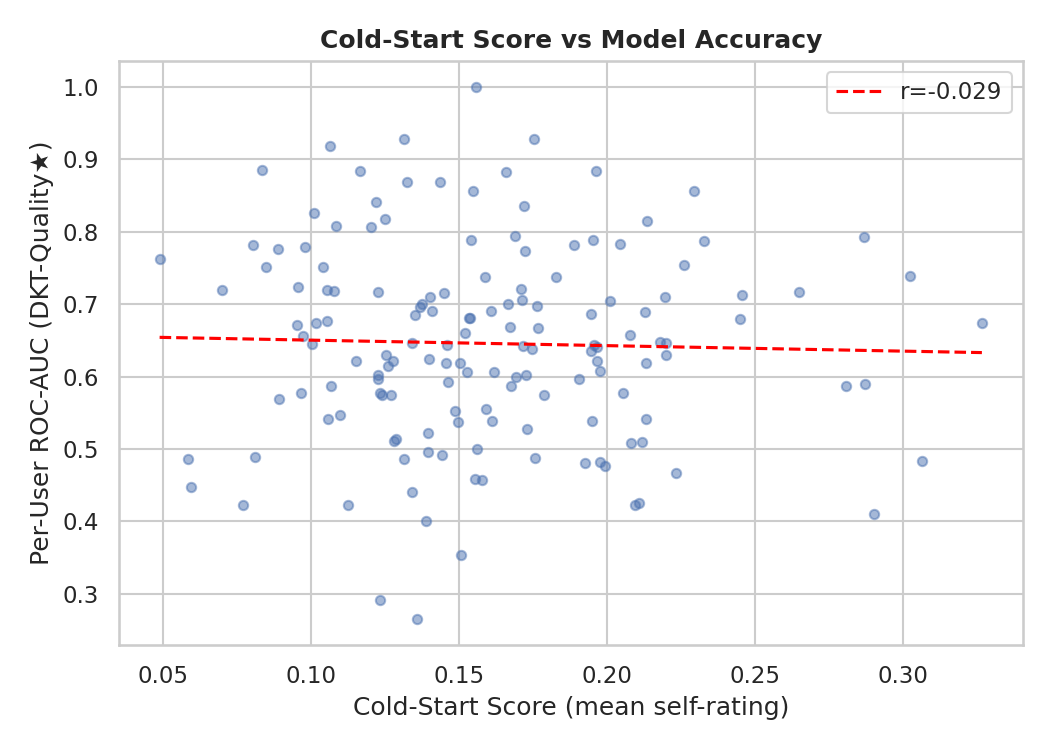
\includegraphics[width=0.95\columnwidth]{coldstart_vs_acc.png}
  \caption{Độ chính xác theo số tương tác -- cold-start được xử lý tốt nhờ EMA fallback.}
  \label{fig:coldstart}
\end{figure}

% ══════════════════════════════════════════════════════════════════
\section{Kiến Trúc Hệ Thống}
\label{sec:system}

\sys{} được xây dựng theo kiến trúc 3 lớp:

\textbf{Lớp dữ liệu:} \texttt{data\_loader.py} nạp 2{,}122 câu hỏi từ \texttt{question\_bank.json}, chuẩn hóa sang schema snake\_case. JSON Schema validate cấu trúc câu hỏi, KC taxonomy, và user profile.

\textbf{Lớp KT/Scoring:} \texttt{competency\_engine.py} quản lý 17 KC và cập nhật skill vector. \texttt{scoring.py} chấm điểm deterministic (MC/TF/Fill). \texttt{kt\_predictor.py} load model DKT và dự đoán mastery.

\textbf{Lớp serving:} FastAPI (\texttt{serving.py}) phục vụ 8 endpoint REST. Streamlit \texttt{app.py} khởi động FastAPI trong background thread và nhúng React SPA vào iframe. React frontend (9 file JSX, không bundler) giao tiếp với backend qua \texttt{fetch}.

Điểm đặc biệt của kiến trúc: React và Python dùng naming convention khác nhau (camelCase vs snake\_case). Normalize boundary được đặt tại hai điểm -- \texttt{\_map\_question()} (Python $\to$ React) và \texttt{\_normalize\_question()} (React $\to$ Python) -- theo nguyên tắc trừu tượng hóa của CT.

% ══════════════════════════════════════════════════════════════════
\section{Thảo Luận}
\label{sec:discussion}

\subsection{CT giúp giải quyết bài toán như thế nào}

Nếu không có phương pháp CT có hệ thống, nhóm có thể mắc vào bẫy ``xây dựng tất cả cùng lúc'' -- kết quả là không hoàn thành module nào. Bước \textit{phân rã} cho phép nhóm song song hóa công việc: trong khi một người xây question bank, người khác thiết kế KT pipeline.

Bước \textit{nhận dạng mẫu} từ EDA (learning curve dốc lên trong 10 tương tác đầu) trực tiếp dẫn đến quyết định thiết kế Stage 1 có 7 câu thay vì ít hơn -- đủ để KT model có lịch sử ý nghĩa trước khi vào Stage 2.

Bước \textit{trừu tượng hóa} KC taxonomy cho phép question bank và KT model hoàn toàn tách biệt -- thêm câu hỏi mới không cần retrain model, chỉ cần tag KC phù hợp.

\subsection{Hạn Chế}

\textbf{Simulation bias:} Toàn bộ dữ liệu KT được sinh bởi IRT -- cùng inductive bias với BKT -- làm kết quả đánh giá thiên lệch. Cần dữ liệu người dùng thực để xác nhận.

\textbf{Sequence length cố định:} Tất cả người dùng có đúng 40 tương tác do question bank bị cap, làm giảm tính tổng quát của mô hình.

\textbf{KT trên Vercel:} Mô hình DKT yêu cầu PyTorch và weights file $>$50MB, không khả thi trên Vercel serverless (timeout 10s). Hệ thống production cần host model riêng.

% ══════════════════════════════════════════════════════════════════
\section{Kết Luận}
\label{sec:conclusion}

Bài báo đã trình bày cách áp dụng tư duy tính toán để xây dựng \sys{} -- hệ thống luyện phỏng vấn IT cá nhân hóa tích hợp Knowledge Tracing. Bốn trụ cột CT (phân rã, nhận dạng mẫu, trừu tượng hóa, thiết kế thuật toán) được vận dụng nhất quán từ phân tích bài toán đến thiết kế thuật toán adaptive và kiến trúc phần mềm.

Kết quả thực nghiệm xác nhận: DKT-Quality đạt PR-AUC~=~0.907, vượt baseline 8.7\% PR-AUC Gain. Cơ chế KT(70\%)~+~EMA(30\%) giải quyết bài toán cold-start hiệu quả. 2-Stage Branching CAT cung cấp trải nghiệm adaptive có cấu trúc.

Hướng phát triển tiếp theo: (1) thu thập dữ liệu người dùng thực để loại bỏ simulation bias; (2) tích hợp LLM để sinh câu hỏi follow-up động; (3) host DKT model trên external service để Vercel app có KT prediction thực sự.

% ── Bibliography ──────────────────────────────────────────────────
\bibliographystyle{IEEEtran}

\begin{thebibliography}{99}

\bibitem{wing2006computational}
J.~M.~Wing, ``Computational thinking,'' \textit{Communications of the ACM}, vol.~49, no.~3, pp.~33--35, 2006.

\bibitem{corbett1994knowledge}
A.~T.~Corbett and J.~R.~Anderson, ``Knowledge tracing: Modeling the acquisition of procedural knowledge,'' \textit{User Modeling and User-Adapted Interaction}, vol.~4, no.~4, pp.~253--278, 1994.

\bibitem{piech2015deep}
C.~Piech \textit{et al.}, ``Deep knowledge tracing,'' in \textit{Advances in Neural Information Processing Systems}, vol.~28, 2015.

\bibitem{pandey2019self}
S.~Pandey and G.~Karypis, ``A self-attentive model for knowledge tracing,'' in \textit{Proc. 12th Int. Conf. Educational Data Mining}, 2019.

\bibitem{embretson2000item}
S.~E.~Embretson and S.~P.~Reise, \textit{Item Response Theory for Psychologists}. Lawrence Erlbaum Associates, 2000.

\bibitem{topdev2024}
TopDev, ``Vietnam IT Market Report 2024,'' TopDev, Tech. Rep., 2024.

\bibitem{wainer2000computerized}
H.~Wainer \textit{et al.}, \textit{Computerized Adaptive Testing: A Primer}, 2nd~ed. Lawrence Erlbaum Associates, 2000.

\bibitem{heffernan2014assistments}
N.~T.~Heffernan and C.~L.~Heffernan, ``The ASSISTments ecosystem,'' \textit{International Journal of Artificial Intelligence in Education}, vol.~24, no.~4, pp.~470--497, 2014.

\end{thebibliography}

\end{document}
